\documentclass{beamer}

\usepackage[UKenglish]{isodate}
\usepackage[utf8]{inputenc}
\usepackage[T1]{fontenc}
\usepackage{textcomp}
\usepackage{listings}
\usepackage{lmodern}
\usepackage{pgf}
\usepackage{tikz}

\usecolortheme{dove}
\setbeamertemplate{navigation symbols}{}
\lstset{frame=lrbt}
\lstdefinelanguage{scala}{
  morekeywords={abstract,case,catch,class,def,%
    do,else,extends,false,final,finally,%
    for,if,implicit,import,match,mixin,%
    new,null,object,override,package,%
    private,protected,requires,return,sealed,%
    super,this,throw,trait,true,try,%
    type,val,var,while,with,yield},
  otherkeywords={=>,<-,<\%,<:,>:,\#,@},
  sensitive=true,
  morecomment=[l]{//},
  morecomment=[n]{/*}{*/},
  morestring=[b]",
  morestring=[b]',
  morestring=[b]"""
}
\lstdefinelanguage{cabal}{
  alsoletter={-},
  morekeywords={name,version,indefinite,exposed-signatures,exposed-modules,build-depends,reexported-modules},
  sensitive=true
}
\usetikzlibrary{arrows,automata,positioning}
\tikzset{
    state/.style={
           rectangle,
           rounded corners,
           draw=black,
           minimum height=1.5em,
           inner sep=2pt,
           text centered,
           },
}


\begin{document}

\title{Modularity and Backpack}
\author{Maciek Makowski (@mmakowski)}

% -------------------------------------------
\frame{\titlepage}

% -------------------------------------------
\begin{frame}{MirageOS}
\makebox[\textwidth][c]{
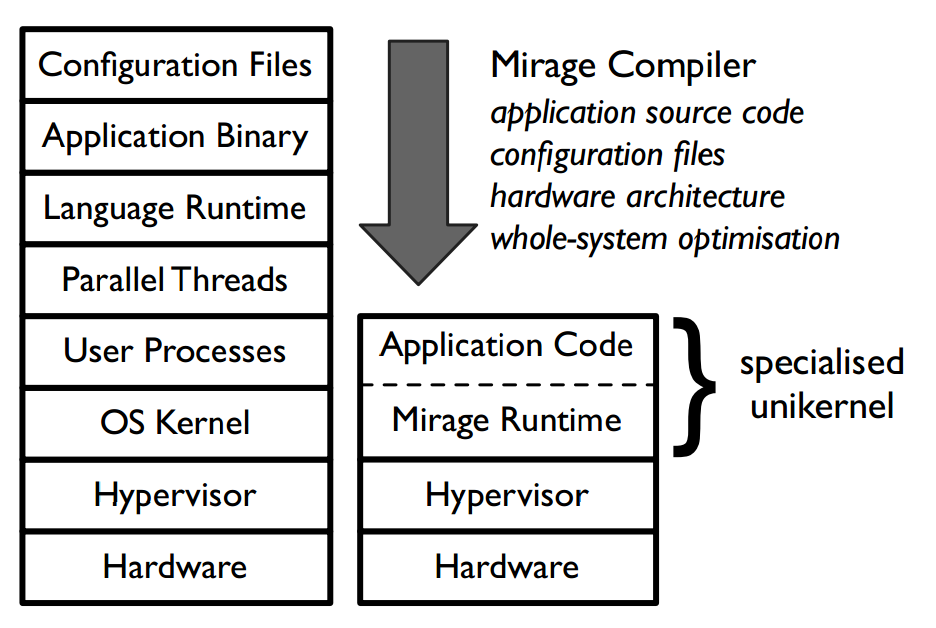
\includegraphics[width=12cm]{unikernel.png}
}
\end{frame}

% -------------------------------------------
\begin{frame}{MirageOS}
\makebox[\textwidth][c]{
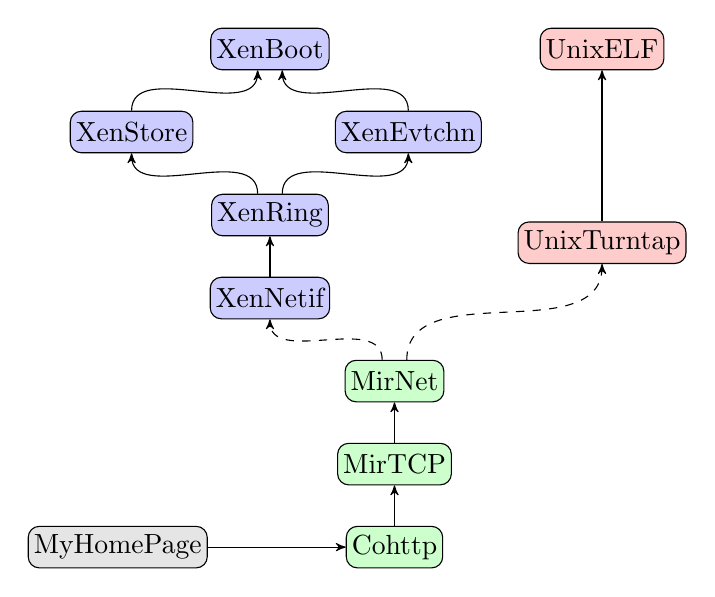
\begin{tikzpicture}[
  ->,>=stealth',
  node distance=3em,
  xen/.style={fill=blue!20},
  unix/.style={fill=red!20},
  mir/.style={fill=green!20}]
\node[state,xen](xenboot){XenBoot};
\node[state,xen,below of=xenboot,xshift=-5em](xenstore){XenStore};
\node[state,xen,below of=xenboot,xshift=5em](xenevtchn){XenEvtchn};
\node[state,xen,below of=xenstore,xshift=5em](xenring){XenRing};
\node[state,xen,below of=xenring](xennetif){XenNetif};
\node[state,mir,below of=xennetif,xshift=4.5em](mirnet){MirNet};
\node[state,mir,below of=mirnet](mirtcp){MirTCP};
\node[state,mir,below of=mirtcp](cohttp){Cohttp};
\node[state,fill=gray!20,left of=cohttp,node distance=10em](myhomepage){MyHomePage};
\node[state,unix,right of=xenboot,node distance=12em](unixelf){UnixELF};
\node[state,unix,below of=unixelf,node distance=7em](unixturntap){UnixTurntap};

\path (myhomepage) edge (cohttp)
      (cohttp) edge (mirtcp)
      (mirtcp) edge (mirnet)
      (mirnet.120) edge[out=90,in=-90,dashed] (xennetif)
      (mirnet.60) edge[out=90,in=-90,dashed] (unixturntap)
      (xennetif) edge (xenring)
      (xenring.120) edge[out=90,in=-90] (xenstore)
      (xenring.60) edge[out=90,in=-90] (xenevtchn)
      (xenstore) edge[out=90,in=-90] (xenboot.240)
      (xenevtchn) edge[out=90,in=-90] (xenboot.300)
      (unixturntap) edge (unixelf);
\end{tikzpicture}
}
\end{frame}

% -------------------------------------------
\begin{frame}{Exhibit 1}{MirageOS}
\begin{quote}
The compiler heavily emphasises static type checking, and the resulting binaries are fast native code with no runtime type information and the module system is among the most powerful in a general-purpose programming language in terms of permitting flexible and safe code reuse and refactoring.
\end{quote}
-- Technical Background of MirageOS
\end{frame}

% -------------------------------------------
\begin{frame}[fragile]{ML Modules}{Structures}
\begin{lstlisting}[language=ML]
structure IntInteger =
  struct
    type integer = int
    val zero = 0
    fun succ n = n + 1
    fun add a b = a + b
    fun mul a b = a * b
  end
\end{lstlisting}
\end{frame}

% -------------------------------------------
\begin{frame}[fragile]{ML Modules}{Signatures}
\begin{lstlisting}[language=ML]
signature INTEGER =
  sig
    type integer
    val zero: integer
    val succ: integer -> integer
    val add: integer -> integer -> integer
    val mul: integer -> integer -> integer
  end
\end{lstlisting}
\end{frame}

% -------------------------------------------
\begin{frame}[fragile]{ML Modules}{Functors}
\begin{lstlisting}[language=ML]
functor RationalFun(I: INTEGER) =
  struct
    type rational = I.integer * I.integer
    fun nom (n, _) = n
    fun denom (_, d) = d
    fun add (n1, d1) (n2, d2) =
      (I.add (I.mul n1 d2) (I.mul n2 d1),
       I.mul d1 d2)
  end
\end{lstlisting}
\begin{lstlisting}[language=ML]
structure IntRational = RationalFun(IntInteger)
\end{lstlisting}
\end{frame}

% -------------------------------------------
\begin{frame}{ML Modules}
\makebox[\textwidth][c]{
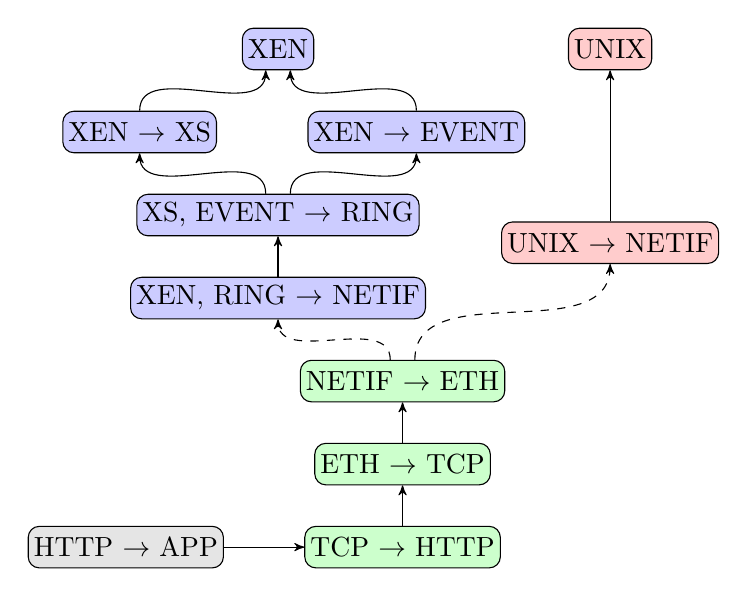
\begin{tikzpicture}[
  ->,>=stealth',
  node distance=3em,
  xen/.style={fill=blue!20},
  unix/.style={fill=red!20},
  mir/.style={fill=green!20}]
\node[state,xen](xenboot){XEN};
\node[state,xen,below of=xenboot,xshift=-5em](xenstore){XEN $\rightarrow$ XS};
\node[state,xen,below of=xenboot,xshift=5em](xenevtchn){XEN $\rightarrow$ EVENT};
\node[state,xen,below of=xenstore,xshift=5em](xenring){XS, EVENT $\rightarrow$ RING};
\node[state,xen,below of=xenring](xennetif){XEN, RING $\rightarrow$ NETIF};
\node[state,mir,below of=xennetif,xshift=4.5em](mirnet){NETIF $\rightarrow$ ETH};
\node[state,mir,below of=mirnet](mirtcp){ETH $\rightarrow$ TCP};
\node[state,mir,below of=mirtcp](cohttp){TCP $\rightarrow$ HTTP};
\node[state,fill=gray!20,left of=cohttp,node distance=10em](myhomepage){HTTP $\rightarrow$ APP};
\node[state,unix,right of=xenboot,node distance=12em](unixelf){UNIX};
\node[state,unix,below of=unixelf,node distance=7em](unixturntap){UNIX $\rightarrow$ NETIF};

\path (myhomepage) edge (cohttp)
      (cohttp) edge (mirtcp)
      (mirtcp) edge (mirnet)
      (mirnet.120) edge[out=90,in=-90,dashed] (xennetif)
      (mirnet.60) edge[out=90,in=-90,dashed] (unixturntap)
      (xennetif) edge (xenring)
      (xenring.120) edge[out=90,in=-90] (xenstore)
      (xenring.60) edge[out=90,in=-90] (xenevtchn)
      (xenstore) edge[out=90,in=-90] (xenboot.240)
      (xenevtchn) edge[out=90,in=-90] (xenboot.300)
      (unixturntap) edge (unixelf);
\end{tikzpicture}
}
\end{frame}

% -------------------------------------------
\begin{frame}[fragile]{Scala}
\begin{lstlisting}[language=Scala,title=trait \textasciitilde\ signature]
trait IntegerSig {
  type Integer
}
\end{lstlisting}
\begin{lstlisting}[language=Scala,title=object \textasciitilde\ structure]
object IntInteger extends IntegerSig {
  type Integer = Int
}
\end{lstlisting}
\begin{lstlisting}[language=Scala,title=class \textasciitilde\ functor]
class RationalFun[I <: IntegerSig](i: I) {
  type Rational = (I#Integer, I#Integer)
}
\end{lstlisting}
\end{frame}

% -------------------------------------------
\begin{frame}[fragile]{Exhibit 2}{tagstream-conduit}
\begin{lstlisting}[language=Haskell]
data Dec builder string = Dec
  { decToS     :: builder -> string
  , decBreak   :: (Char -> Bool) -> string ->
                  (string,string)
  , decBuilder :: string -> builder
  , decDrop    :: Int -> string -> string
  , decEntity  :: string -> Maybe string
  , decUncons  :: string -> Maybe (Char,string)
  }
\end{lstlisting}
\end{frame}

% -------------------------------------------
\begin{frame}[fragile]{Exhibit 3}{tagsoup}
\begin{lstlisting}[language=Haskell]
class (Typeable a, Eq a) => StringLike a where
    empty      :: a
    cons       :: Char -> a -> a
    uncons     :: a -> Maybe (Char, a)
    toString   :: a -> String
    fromString :: String -> a
    -- [...]
\end{lstlisting}
\end{frame}

% -------------------------------------------
\begin{frame}[fragile]{Backpack}{Modules}
\begin{lstlisting}[language=Haskell]
module IntegerInt where

type Integer = Int

zero = 0
succ = (+1)
add = (+)
mul = (*)
\end{lstlisting}
\end{frame}

% -------------------------------------------
\begin{frame}[fragile]{Backpack}{Signatures}
\begin{lstlisting}[language=Haskell]
module IntegerSig where

data Integer

zero :: Integer
succ :: Integer
add  :: Integer -> Integer -> Integer
mul  :: Integer -> Integer -> Integer
\end{lstlisting}
\end{frame}

% -------------------------------------------
\begin{frame}[fragile]{Backpack}{Modules}
\begin{lstlisting}[language=Haskell]
module Rational where

import qualified IntegerSig as I

data Rational = R I.Integer I.Integer

nom (R n _) = n
denom (R _ d) = d
add (R n1 d1) (R n2 d2) =
  R (I.add (I.mul n1 d2) (I.mul n2 d1))
    (I.mul d1 d2)
\end{lstlisting}
\end{frame}

% -------------------------------------------
\begin{frame}[fragile]{Backpack}{Cabal packages}
\begin{lstlisting}[language=Cabal,title=Integer implementation package]
name:            integer-int
exposed-modules: IntegerInt
\end{lstlisting}
\end{frame}

% -------------------------------------------
\begin{frame}[fragile]{Backpack}{Cabal packages}
\begin{lstlisting}[language=Cabal,title=Integer signature package]
name:               integer-sig
version:            1.0
indefinite:         True
exposed-signatures: IntegerSig
\end{lstlisting}
\end{frame}

% -------------------------------------------
\begin{frame}[fragile]{Backpack}{Cabal packages}
\begin{lstlisting}[language=Cabal,title=Rational ``functor'' package]
name:            rational
indefinite:      True
build-depends:   integer-sig-1.0
exposed-modules: Rational
\end{lstlisting}
\end{frame}

% -------------------------------------------
\begin{frame}[fragile]{Backpack}{Mixing in}
\begin{lstlisting}[language=Cabal,title=Rationals based on Integers]
name:               rational-int
build-depends:
  integer (IntegerInt as IntegerSig),
  rational
reexported-modules: Rational as RationalInt
\end{lstlisting}
\end{frame}

% -------------------------------------------
\begin{frame}{Backpack}{Package hierarchy}
\makebox[\textwidth][c]{
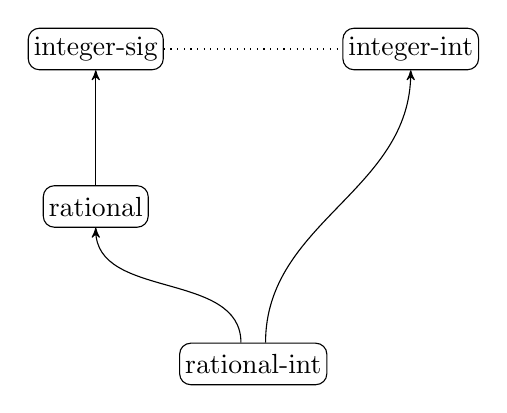
\begin{tikzpicture}[->,>=stealth']
\node[state](integersig){integer-sig};
\node[state,right of=integersig,node distance=4cm](integerint){integer-int};
\node[state,below of=integersig,node distance=2cm](rational){rational};
\node[state,below of=rational,node distance=2cm,xshift=2cm](rationalint){rational-int};
\path (rationalint.120) edge[out=90,in=-90] (rational)
      (rationalint.60) edge[out=90,in=-90] (integerint)
      (rational) edge (integersig);
\draw[dotted,-] (integersig) -- (integerint);
\end{tikzpicture}
}
\end{frame}

% -------------------------------------------
\begin{frame}[fragile]{Instantiation Semantics}
\begin{lstlisting}[language=ML]
functor RationalFunD(I: INTEGER) =
  struct
    datatype rational =
      R of I.integer * I.integer
    val zero = R (I.zero, I.succ I.zero)
  end
structure R1 = RationalFunD(IntInteger)
structure R2 = RationalFunD(IntInteger)
\end{lstlisting}
Is R1.rational the same type as R2.rational?
\begin{itemize}
\item \textit{generative}: no
\item \textit{applicative}: yes
\end{itemize}
\end{frame}

% -------------------------------------------
\begin{frame}[fragile]{Backpack}{Recursive linking}
\makebox[\textwidth][c]{
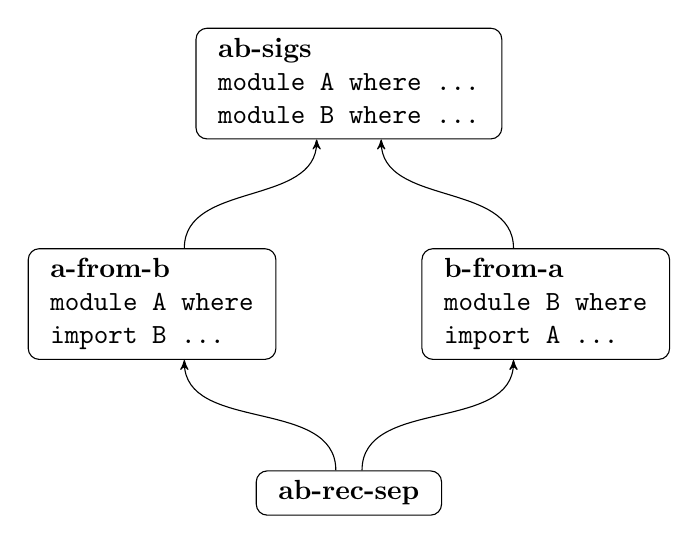
\begin{tikzpicture}[->,>=stealth']
\node[state](absigs){
  \begin{tabular}{l}
    \textbf{ab-sigs}\\
    \texttt{module A where ...}\\
    \texttt{module B where ...}
  \end{tabular}
};
\node[state,below of=absigs,node distance=2.8cm,xshift=-2.5cm](afromb){
  \begin{tabular}{l}
    \textbf{a-from-b}\\
    \texttt{module A where}\\
    \texttt{import B ...}
  \end{tabular}
};
\node[state,below of=absigs,node distance=2.8cm,xshift=2.5cm](bfroma){
  \begin{tabular}{l}
    \textbf{b-from-a}\\
    \texttt{module B where}\\
    \texttt{import A ...}
  \end{tabular}
};
\node[state,below of=absigs,node distance=5.2cm](abrecsep){
  \begin{tabular}{l}
    \textbf{ab-rec-sep}
  \end{tabular}
};
\path (afromb.60) edge[out=90,in=-90] (absigs.240)
      (bfroma.120) edge[out=90,in=-90] (absigs.300)
      (abrecsep.120) edge[out=90,in=-90] (afromb.300)
      (abrecsep.60) edge[out=90,in=-90] (bfroma.240);
\end{tikzpicture}
}
\end{frame}

% -------------------------------------------
\begin{frame}[fragile]{Module Systems}{Features}
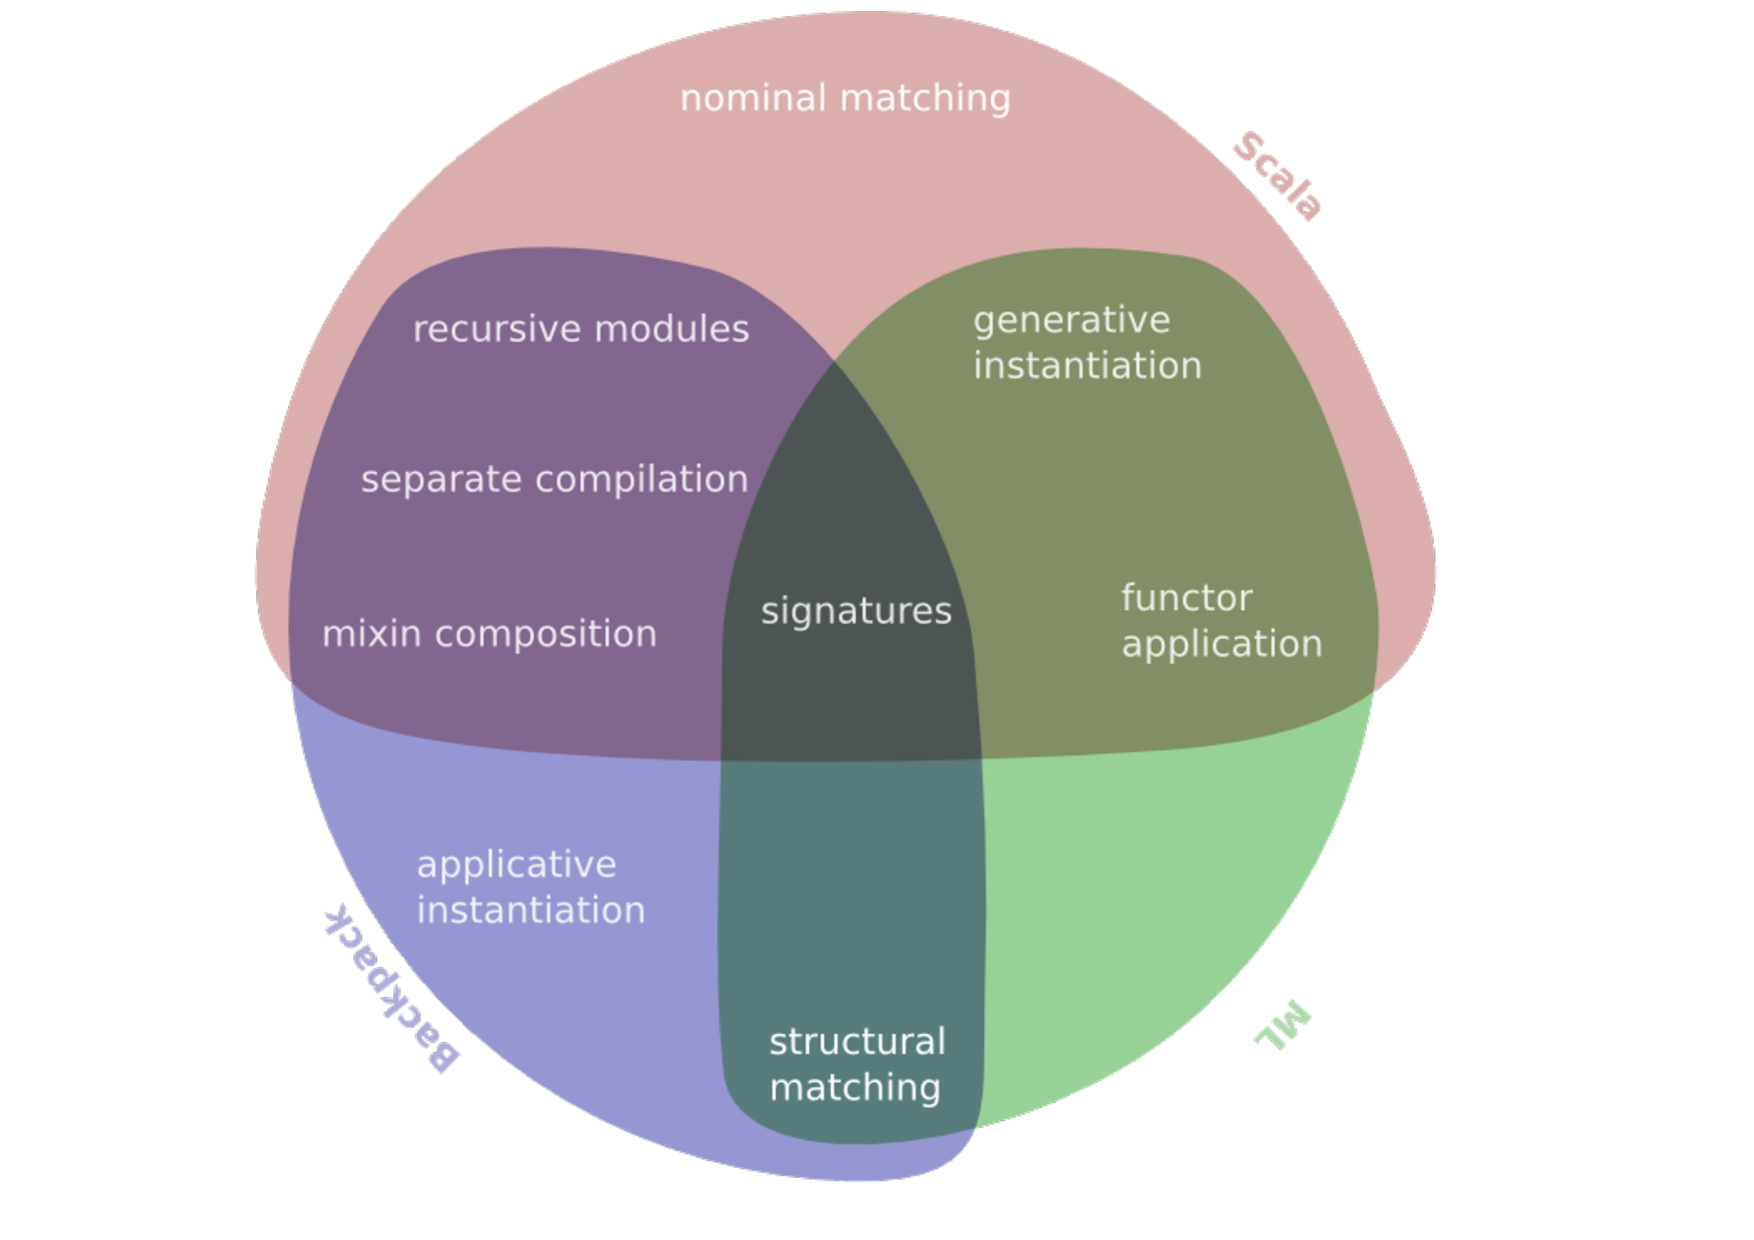
\includegraphics[width=12cm]{features.pdf}
\end{frame}

% -------------------------------------------
\begin{frame}[fragile]{More}
\begin{itemize}
\item blog.ezyang.com (including comments)
\item Edward Yang's \textit{Haskell Implementor's Workshop} talk
\item The Backpack paper
\item papers by Derek Dreyer (e.g. MixML)
\end{itemize}
\end{frame}

\end{document}
